% =========================================================
% EmPath: Multimodal Pain Intensity Detection
% Journal Paper Style (two-column, Frontiers/IEEE style)
% Komala Belur Srinivas — Hofstra University
% Compile: pdflatex → biber → pdflatex × 2
%          (Overleaf: engine pdfLaTeX + biber)
% =========================================================

\documentclass[10pt, twocolumn]{article}

% ─── Page Layout ────────────────────────────────────────
\usepackage[
  top=0.9in, bottom=1.0in,
  left=0.75in, right=0.75in,
  columnsep=0.25in,
  headheight=13.6pt
]{geometry}
\usepackage{stfloats}   % allows figure* at [b]

% ─── Fonts & Typography ─────────────────────────────────
\usepackage{newtxtext, newtxmath}
\usepackage{microtype}
\usepackage[T1]{fontenc}
\usepackage[utf8]{inputenc}

% ─── Colors ─────────────────────────────────────────────
\usepackage[dvipsnames, table]{xcolor}
\definecolor{journalblue}{RGB}{0,68,115}
\definecolor{journalteal}{RGB}{0,120,112}
\definecolor{sectionrule}{RGB}{0,100,140}
\definecolor{abstractbg}{RGB}{242,248,252}
\definecolor{codebackground}{RGB}{248,248,248}
\definecolor{codekeyword}{RGB}{0,0,160}
\definecolor{codecomment}{RGB}{90,90,90}
\definecolor{codestring}{RGB}{150,20,20}
\definecolor{codeborder}{RGB}{180,180,180}

% ─── Section Formatting ─────────────────────────────────
\usepackage{titlesec}
\titleformat{\section}
  {\normalfont\large\bfseries\color{journalblue}}
  {\thesection.}{0.5em}{}[{\color{sectionrule}\titlerule[0.5pt]}]
\titleformat{\subsection}
  {\normalfont\normalsize\bfseries}
  {\thesubsection}{0.5em}{}
\titleformat{\subsubsection}
  {\normalfont\normalsize\itshape\bfseries}
  {\thesubsubsection}{0.5em}{}
\titleformat{\paragraph}[runin]
  {\normalfont\normalsize\bfseries}
  {}{0em}{}[.]
\titlespacing{\section}{0pt}{10pt plus 2pt minus 1pt}{4pt}
\titlespacing{\subsection}{0pt}{8pt plus 2pt minus 1pt}{2pt}
\titlespacing{\subsubsection}{0pt}{6pt plus 1pt}{1pt}

% ─── Headers & Footers ──────────────────────────────────
\usepackage{fancyhdr}
\pagestyle{fancy}
\fancyhf{}
\renewcommand{\headrulewidth}{0.4pt}
\fancyhead[LE,LO]{\footnotesize\textit{Belur Srinivas}}
\fancyhead[RE,RO]{\footnotesize\textit{EmPath: Multimodal Pain Intensity Detection}}
\fancyfoot[CE,CO]{\small\thepage}
\fancypagestyle{firstpage}{
  \fancyhf{}
  \renewcommand{\headrulewidth}{0pt}
  \fancyfoot[CE,CO]{\small\thepage}
}

% ─── Bibliography ───────────────────────────────────────
\usepackage[american]{babel}
\usepackage{csquotes}
\usepackage[style=apa,sortcites=true,sorting=nyt,backend=biber]{biblatex}
\addbibresource{references.bib}

% ─── Graphics & Diagrams ────────────────────────────────
\usepackage{tikz}
\usepackage{pgfplots}
\usepackage{pgfplotstable}
\pgfplotsset{compat=1.18}
\usetikzlibrary{
  shapes.geometric, arrows.meta, positioning,
  calc, decorations.pathreplacing, fit, backgrounds,
  matrix, chains, scopes
}

% ─── Tables ─────────────────────────────────────────────
\usepackage{booktabs}
\usepackage{multirow}
\usepackage{array}
\usepackage{tabularx}
\usepackage{longtable}

% ─── Code Listings ──────────────────────────────────────
\usepackage{listings}
\usepackage{float}  % enables float=t option on lstlisting
\lstdefinestyle{pythonstyle}{
  language=Python,
  backgroundcolor=\color{codebackground},
  basicstyle=\ttfamily\scriptsize,
  keywordstyle=\color{codekeyword}\bfseries,
  commentstyle=\color{codecomment}\itshape,
  stringstyle=\color{codestring},
  numberstyle=\tiny\color{gray},
  numbers=left,
  numbersep=5pt,
  stepnumber=1,
  showstringspaces=false,
  breaklines=true,
  breakatwhitespace=false,
  frame=single,
  rulecolor=\color{codeborder},
  tabsize=4,
  captionpos=b,
  xleftmargin=10pt,
  framexleftmargin=10pt,
}
\lstset{style=pythonstyle}
\renewcommand{\lstlistingname}{Code Snippet}  % match in-text "Code Snippet N" references

% ─── Math ───────────────────────────────────────────────
\usepackage{amsmath}
\usepackage{amssymb}

% ─── Misc ───────────────────────────────────────────────
\usepackage{graphicx}
\usepackage{caption}
\captionsetup{font=small, labelfont=bf, labelsep=period}
\captionsetup[table]{position=top}
\usepackage{mdframed}

% ─── Float control ──────────────────────────────────────
% Prevent floats accumulating past section boundaries and
% appearing after the bibliography in two-column layout.
\usepackage{placeins}   % provides \FloatBarrier
% Allow more floats per page and lower the threshold
% at which LaTeX outputs a float-only page.
\setcounter{topnumber}{4}
\setcounter{bottomnumber}{2}
\setcounter{totalnumber}{6}
\renewcommand{\topfraction}{0.85}
\renewcommand{\bottomfraction}{0.5}
\renewcommand{\textfraction}{0.10}
\renewcommand{\floatpagefraction}{0.80}

% ─── Hyperlinks ─────────────────────────────────────────
\usepackage[colorlinks=true, linkcolor=journalblue,
            citecolor=journalteal, urlcolor=journalblue]{hyperref}

% ─── Custom Keywords command ────────────────────────────
\newcommand{\keywords}[1]{%
  \vspace{0.5em}
  \noindent\textbf{Keywords:} \textit{#1}
  \vspace{1em}
}

% =========================================================
\begin{document}
\thispagestyle{firstpage}

% ─── Full-width title block (before two columns) ────────
\twocolumn[{
  \begin{center}
    \vspace*{0.3em}
    {\color{journalblue}\rule{\textwidth}{1pt}}
    \vspace{0.8em}

    {\LARGE\bfseries\color{journalblue}
      EmPath: Multimodal Pain Intensity Detection\\[0.3em]
      Using Biosignals and Facial Landmarks}

    \vspace{0.8em}

    {\large\textbf{Komala Belur Srinivas}}\\[0.3em]
    {\small Department of Computer Science, Hofstra University, Hempstead, NY, USA}\\
    {\small Capstone Project, Supervisor: Dr.~Purna Prasad, May 2026}

    \vspace{0.8em}
    {\color{journalblue}\rule{\textwidth}{0.5pt}}
    \vspace{0.5em}
  \end{center}

  \begin{mdframed}[backgroundcolor=abstractbg, linecolor=journalblue,
                   linewidth=0.6pt, innerleftmargin=8pt, innerrightmargin=8pt,
                   innertopmargin=6pt, innerbottommargin=6pt]
    \noindent{\small\textbf{\color{journalblue}Abstract:} %
    This study presents EmPath, a multimodal machine learning system for discriminating
    between two adjacent pain intensity levels (PA2 and PA3) using the BioVid Heat Pain
    Database. Physiological signals (galvanic skin response, electrocardiogram,
    electromyography) and facial landmark trajectories extracted via MediaPipe FaceMesh
    were processed into 35 biosignal and 22 landmark features across 2,680 trials from
    67 thermally reactive participants. A stacked generalization framework combining two
    base Random Forest classifiers with a Logistic Regression meta-learner was evaluated
    under Leave-One-Subject-Out (LOSO) cross-validation. The fusion model achieved 65.3\%
    accuracy (\textit{SD} = 14.1\%, AUC = 0.719, \textit{F}$_1$ = 0.653), outperforming
    the biosignal-only baseline (63.1\% $\pm$ 11.6\%) and landmark-only baseline
    (61.4\% $\pm$ 13.1\%). SHAP analysis identified \texttt{gsr\_slope} as the dominant
    biosignal predictor (mean $|\text{SHAP}|$ = 0.0372), and \texttt{mouth\_height\_std}
    as the dominant facial predictor (mean $|\text{SHAP}|$ = 0.0289). An ablation study
    across 26 architectural variants (including deep learning, graph neural networks,
    domain-adversarial networks, and temporal velocity features) confirmed the stacked
    fusion configuration as optimal. These findings demonstrate that multimodal fusion
    with person-specific normalization provides consistent, albeit modest, improvements
    over unimodal baselines for adjacent-level pain intensity classification, while
    underscoring the fundamental difficulty of subject-independent affective state
    discrimination.}
  \end{mdframed}
  \vspace{0.5em}
  \noindent\textbf{\small Keywords:} {\small\textit{pain detection; multimodal fusion;
    biosignals; facial landmarks; stacked generalization; leave-one-subject-out; SHAP;
    BioVid}}
  \vspace{1.2em}
  {\color{journalblue}\rule{\textwidth}{0.5pt}}
  \vspace{1.2em}
}]

% =========================================================
\section{Introduction}
\label{sec:intro}
% =========================================================

Pain is the most common reason patients seek medical care, yet its assessment remains
predominantly subjective, relying on self-report instruments such as visual analog scales
(VAS) or numeric rating scales (NRS; \cite{Jensen2003}). This dependence on verbal
communication creates a fundamental gap in clinical practice: patients who cannot reliably
self-report (including those under intensive care sedation, individuals with advanced
dementia, neonates, and patients with severe communication disorders) may receive
inadequate analgesia because clinicians lack objective tools to quantify their pain states
(\cite{Lichtner2014}; \cite{Puntillo2009}). Automated, non-invasive pain assessment using
physiological and behavioral signals represents a critical research frontier with direct
clinical consequences.

The autonomic nervous system responds to nociceptive stimulation through measurable changes
in galvanic skin response (GSR), heart rate variability (HRV), and electromyographic
activity (EMG; \cite{Loggia2011}). Simultaneously, pain produces characteristic facial
muscle activations that are largely involuntary and observable across cultural contexts
(\cite{Ekman1978}; \cite{Prkachin2008}). These two signal streams (physiological and
behavioral) carry complementary information: biosignals capture systemic autonomic
activation, while facial movements encode the expressive component of the pain experience.
Combining them through multimodal fusion should, in principle, yield more reliable pain
estimates than either channel alone (\cite{Werner2019}).

The BioVid Heat Pain Database (\cite{Walter2013}) provides a standardized benchmark for
developing such systems. The database contains synchronized physiological signals and video
recordings of 87 participants exposed to precisely calibrated thermal stimuli at four
intensity levels (PA1--PA4), with a neutral baseline (BL). Discriminating between adjacent
intensity levels, particularly PA2 and PA3, which differ by approximately one degree
Celsius, represents a particularly challenging subproblem that tests the sensitivity of
automated methods to subtle changes in pain magnitude.

Despite growing interest in automated pain recognition, several methodological limitations
pervade the existing literature. First, many published systems evaluate on random train/test
splits, which allow models to memorize individual physiological baselines and inflate
accuracy through subject identity leakage rather than genuine pain discrimination
(\cite{Gruss2015}). Second, deep learning architectures, which dominate contemporary
benchmarks, frequently require more subjects than BioVid provides to generalize across
individuals (\cite{Kachele2015}). Third, few studies systematically compare modality
contributions or apply rigorous feature attribution methods to identify which physiological
signals actually drive classification decisions (\cite{Tavakolian2020}).

The present work addresses these limitations through four specific contributions:

\begin{enumerate}
  \item We implement and evaluate a stacked generalization framework that combines Random
        Forest models trained on biosignal and facial landmark features respectively, using
        a Logistic Regression meta-learner to integrate modality-specific probability
        estimates.
  \item We evaluate exclusively under LOSO cross-validation on the 67 thermally reactive
        subjects in BioVid, providing a strict test of subject-independent generalization.
  \item We conduct a comprehensive ablation study across 26 architectural variants spanning
        deep learning (TCN, MLP, R3D-18), foundation models (BIOT, PainFormer, Tiny-BioMoE),
        graph neural networks, domain-adversarial networks, and temporal velocity approaches.
  \item We apply SHAP TreeExplainer analysis to both base models to identify which features
        drive classification decisions, providing physiologically interpretable insight into
        what the system is learning.
\end{enumerate}

Section~\ref{sec:related} reviews related work in biosignal-based pain detection, facial
action coding, and multimodal fusion. Section~\ref{sec:method} describes the dataset,
feature extraction pipelines, model architecture, and evaluation protocol.
Section~\ref{sec:results} presents quantitative results, ablation findings, and feature
importance analyses. Section~\ref{sec:discussion} interprets the results in light of
physiological theory and existing benchmarks. Section~\ref{sec:limitations} discusses
limitations and future directions. Section~\ref{sec:conclusion} concludes.

% =========================================================
\section{Related Work}
\label{sec:related}
% =========================================================

\subsection{Biosignal-Based Pain Detection}

The use of physiological signals for automated pain assessment has a substantial literature
spanning several decades. Early work relied on simple summary statistics of GSR and heart
rate, demonstrating that autonomic arousal systematically increases with pain intensity
(\cite{Loggia2011}). More recent approaches have adopted machine learning frameworks to
learn non-linear mappings from multivariate feature vectors to pain labels.
\textcite{Tavakolian2020} demonstrated that frequency-domain HRV features, combined with
skin conductance level features, achieve approximately 60\% accuracy for two-class adjacent
pain discrimination on BioVid under LOSO evaluation, a number that contextualizes our
findings. \textcite{Kachele2015} systematically evaluated support vector machines, random
forests, and Gaussian processes on BioVid biosignals, reporting that cross-subject
generalization is substantially lower than within-subject performance, confirming the
difficulty of the subject-independent evaluation protocol.

\textcite{Gkikas2023} provided a comprehensive review of automated pain estimation from
physiological and behavioral cues, noting that most high-accuracy systems exploit
subject-level context and that truly subject-independent accuracy remains bounded below
70\% for adjacent pain levels on BioVid. This observation is consistent with our findings
and motivates person-specific normalization as a preprocessing strategy.

Recent work has explored foundation models pretrained on large biosignal corpora.
BIOT (\cite{Yang2023}), PainFormer, and Tiny-BioMoE represent this paradigm. However,
our experiments demonstrate that fine-tuning these models on BioVid's 67-subject LOSO
regime yields results below 57\%, suggesting substantial distribution mismatch between
pretraining corpora and heat-pain-elicited physiological signals.

\subsection{Facial Action Coding and Landmark-Based Pain Recognition}

The facial expression of pain has been systematically characterized through the Facial
Action Coding System (FACS; \cite{Ekman1978}), which decomposes facial muscle contractions
into discrete Action Units (AUs). Pain-relevant AUs include AU4 (brow lowering), AU6
(cheek raiser), AU9 (nose wrinkler), AU10 (upper lip raiser), AU25 (lip parting), and
AU43 (eyes closed), constituting the Pain Face (\cite{Prkachin2008}).

Computer vision approaches to facial pain recognition have progressed from handcrafted AU
classifiers (\cite{Lucey2011}) to convolutional neural networks (\cite{Rodriguez2017}).
The shift toward landmark-based representations using facial keypoints from MediaPipe
FaceMesh (\cite{Lugaresi2019}) offers a complementary approach: rather than modeling
pixel-level texture, these methods characterize the geometric configuration of facial
structures, providing scale and illumination invariance while encoding clinically
interpretable deformations.

\subsection{Multimodal Fusion}

Combining biosignal and visual modalities for pain recognition is a relatively young area.
\textcite{Gruss2015} evaluated early fusion of EMG, GSR, and video-based AU features on
BioVid, finding that fusion outperforms either modality alone within subjects, but that
the advantage diminishes under cross-subject protocols.

More recent work has explored transformer-based fusion. The CrossMod-Transformer
(\cite{Farmani2025}) achieves 87.5\% accuracy on BioVid using cross-modal attention, though
this result is evaluated on all 87 subjects including the 20 non-reactive individuals;
restricted to reactive subjects, the task difficulty increases substantially.

Stacked generalization, introduced by \textcite{Wolpert1992} and formalized by
\textcite{Breiman1996}, offers an alternative fusion strategy that avoids the need to
align heterogeneous feature representations in a shared embedding space. Each
modality-specific base model produces calibrated probability estimates, which the
meta-learner combines. This approach is particularly well-suited to settings where the
number of training examples per fold is small, reducing the risk of overfitting the fusion
layer.

\subsection{Domain Adaptation for Cross-Subject Generalization}

A fundamental challenge in subject-independent affective computing is physiological
variability between individuals (\cite{Turk2010}). Domain-Adversarial Neural Networks
(DANN; \cite{Ganin2016}) append a gradient-reversal layer to enforce domain-invariant
representations. Our experiments demonstrate that DANN applied to BioVid biosignals
achieves 61.6\% under LOSO-67, improving to 64.7\% when stacked with landmark RF
predictions, but failing to exceed the non-adversarial baseline (65.3\%).

% =========================================================
\section{Method}
\label{sec:method}
% =========================================================

\subsection{Dataset}

The BioVid Heat Pain Database (\cite{Walter2013}) was collected at the University of
Tübingen, Germany. Eighty-seven healthy adult participants (44 women, 43 men; age range
18--65 years; $M_{\text{age}}$ = 41.0, $SD$ = 13.8) received heat pain stimuli of varying
intensities while synchronized physiological signals and video recordings were captured.
Biosignals were recorded at 512~Hz and include GSR from the hand, three-lead ECG, two
trapezius EMG channels, and one zygomaticus EMG channel. Video was captured at 25~fps.

The dataset comprises five stimulus conditions: baseline (BL) and four pain levels
(PA1--PA4). We restrict analysis to PA2 versus PA3, the most challenging adjacent
pair, because (1) this binary discrimination task is standard in the BioVid literature
(\cite{Kachele2015}), (2) the small inter-class difference ($\approx$1°C) maximizes
discriminative difficulty, and (3) binary classification provides a clean framework for
assessing feature informativeness.

To the best of the authors' knowledge, no prior published work has reported
subject-independent LOSO accuracy specifically for the PA2 versus PA3 boundary on the 67
reactive subjects subset of BioVid, making EmPath the first reported result on this
evaluation protocol.

\subsubsection{Subject Reactivity Filtering}

Twenty of the 87 participants exhibit no measurable physiological reaction to heat
stimulus: their GSR, ECG, and EMG signals are effectively flat across all pain conditions.
Including these non-reactive subjects introduces examples where features contain no
discriminative information. Consistent with recommendations in the BioVid methodology
documentation (\cite{Walter2013}) and community protocols (\cite{Gruss2015}), we exclude
these 20 non-reactive subjects and conduct all experiments on the remaining 67 reactive
participants.

Table~\ref{tab:dataset} summarizes the dataset composition after filtering. The 67 retained
subjects contribute 40 stimulus trials each (20 PA2, 20 PA3), yielding 2,680 samples.
Classes are exactly balanced: 1,340 PA2 and 1,340 PA3 samples.

\begin{table}[ht]
\centering
\caption{BioVid Heat Pain Database: Composition After Reactivity Filtering}
\label{tab:dataset}
\small
\begin{tabular}{lrr}
\toprule
\textbf{Category} & \textbf{Count} & \textbf{Notes} \\
\midrule
Total enrolled subjects & 87 & Original database \\
Non-reactive (excluded) & 20 & No physiological response \\
Reactive subjects (used) & 67 & All analyses on this subset \\
\midrule
PA2 samples & 1,340 & $\approx$43°C stimulus \\
PA3 samples & 1,340 & $\approx$44°C stimulus \\
Total samples & 2,680 & Perfectly balanced \\
\midrule
Samples per subject & 40 & 20 PA2 $+$ 20 PA3 \\
Video frame rate & 25~fps & 5.5~s trial window \\
Biosignal sample rate & 512~Hz & GSR, ECG, EMG \\
\bottomrule
\end{tabular}
\end{table}

Figure~\ref{fig:pipeline} illustrates the end-to-end data pipeline.

\begin{figure*}[tbp]
\centering
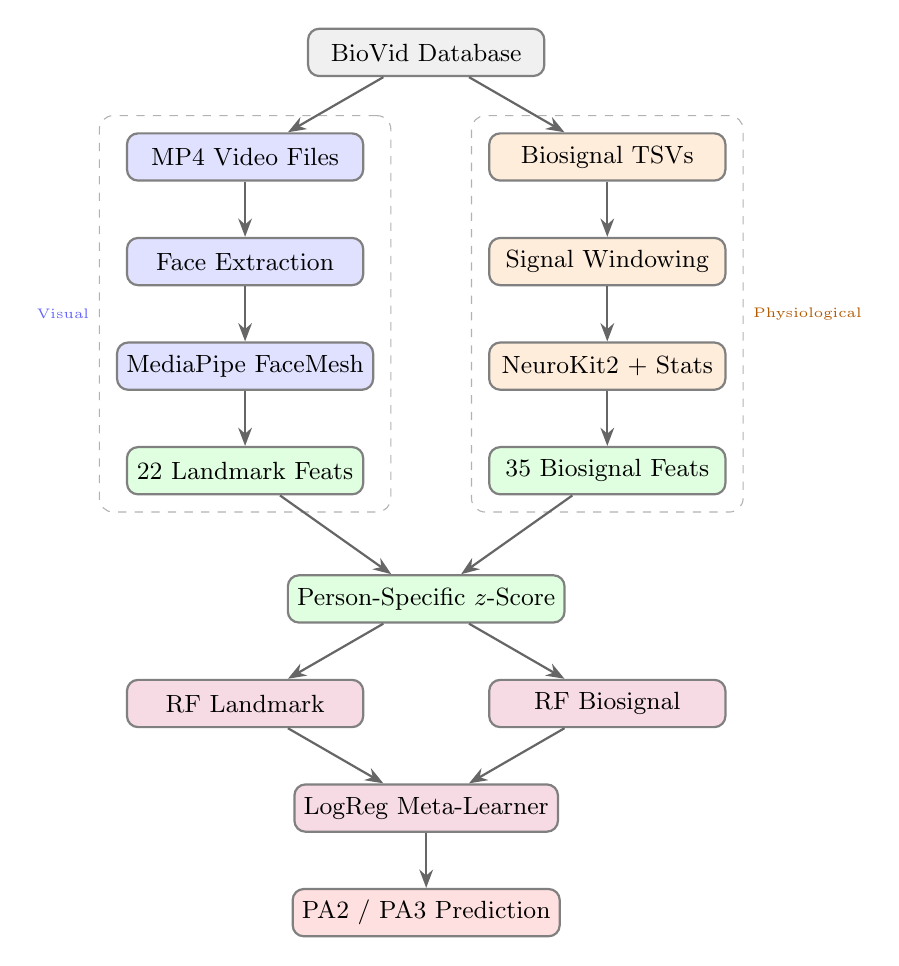
\begin{tikzpicture}[
  node distance=0.5cm and 1.4cm,
  block/.style={
    rectangle, rounded corners=4pt,
    minimum width=3.0cm, minimum height=0.6cm,
    text centered, font=\small,
    draw=black!50, thick
  },
  rawblock/.style={block, fill=gray!12},
  vidblock/.style={block, fill=blue!12},
  bioblock/.style={block, fill=orange!14},
  featblock/.style={block, fill=green!12},
  modelblock/.style={block, fill=purple!14},
  outblock/.style={block, fill=red!12},
  arrow/.style={-Stealth, thick, black!60},
  groupbox/.style={draw=black!30, rounded corners=5pt, dashed, inner sep=6pt}
]
\node[rawblock] (biovid) {BioVid Database};
\node[vidblock,  below=0.7cm of biovid, xshift=-2.3cm] (video)  {MP4 Video Files};
\node[bioblock,  below=0.7cm of biovid, xshift= 2.3cm] (biosig) {Biosignal TSVs};
\node[vidblock,  below=0.7cm of video]  (faces)     {Face Extraction};
\node[bioblock,  below=0.7cm of biosig] (sigwin)    {Signal Windowing};
\node[vidblock,  below=0.7cm of faces]  (mediapipe) {MediaPipe FaceMesh};
\node[bioblock,  below=0.7cm of sigwin] (nk2)       {NeuroKit2 + Stats};
\node[featblock, below=0.7cm of mediapipe] (lmfeat) {22 Landmark Feats};
\node[featblock, below=0.7cm of nk2]       (biofeat) {35 Biosignal Feats};
\node[featblock, below=1.0cm of lmfeat, xshift=2.3cm] (norm) {Person-Specific $z$-Score};
\node[modelblock, below=0.7cm of norm, xshift=-2.3cm] (rflm)  {RF Landmark};
\node[modelblock, below=0.7cm of norm, xshift= 2.3cm] (rfbio) {RF Biosignal};
\node[modelblock, below=0.7cm of rflm, xshift=2.3cm] (meta) {LogReg Meta-Learner};
\node[outblock, below=0.7cm of meta] (out) {PA2 / PA3 Prediction};
\draw[arrow] (biovid) -- (video);
\draw[arrow] (biovid) -- (biosig);
\draw[arrow] (video)   -- (faces);
\draw[arrow] (biosig)  -- (sigwin);
\draw[arrow] (faces)   -- (mediapipe);
\draw[arrow] (sigwin)  -- (nk2);
\draw[arrow] (mediapipe) -- (lmfeat);
\draw[arrow] (nk2)       -- (biofeat);
\draw[arrow] (lmfeat)  -- (norm);
\draw[arrow] (biofeat) -- (norm);
\draw[arrow] (norm) -- (rflm);
\draw[arrow] (norm) -- (rfbio);
\draw[arrow] (rflm)  -- (meta);
\draw[arrow] (rfbio) -- (meta);
\draw[arrow] (meta)  -- (out);
\begin{scope}[on background layer]
  \node[groupbox, fit=(video)(faces)(mediapipe)(lmfeat),
        label={[font=\tiny,text=blue!60]left:Visual}] {};
  \node[groupbox, fit=(biosig)(sigwin)(nk2)(biofeat),
        label={[font=\tiny,text=orange!70!black]right:Physiological}] {};
\end{scope}
\end{tikzpicture}
\caption{End-to-end data pipeline from BioVid raw files to pain intensity prediction.
The visual branch (left, blue) extracts geometric facial landmark features;
the physiological branch (right, orange) extracts time-series statistics from biosignals.
Both branches converge at person-specific normalization before training the stacked
generalization framework.}
\label{fig:pipeline}
\end{figure*}

\subsection{Biosignal Feature Extraction}

\subsubsection{Signal Preprocessing}

For each trial, the 5.5-second biosignal window corresponding to the pain stimulus was
extracted from the raw TSV files using sample onset indices provided in the BioVid metadata
(\texttt{samples.csv}). Signals were already hardware-filtered and provided in physical
units (microsiemens for GSR, millivolts for ECG, normalized units for EMG channels). No
additional bandpass filtering was applied to preserve the full frequency content for feature
computation.

\subsubsection{Feature Computation}

Thirty-five scalar features were extracted from each 5.5-second window across four
physiological domains (see Table~\ref{tab:features}).
Code Snippet~\ref{lst:gsr_slope} shows the implementation of two key features:
\texttt{gsr\_slope} (linear rate of change of skin conductance) and
\texttt{gsr\_shannon} (Shannon entropy of the conductance distribution).

\begin{lstlisting}[caption={GSR slope and Shannon entropy extraction from a single trial window. \texttt{gsr\_vals} is a 1-D NumPy array of skin conductance values (microsiemens) over 5.5 seconds.}, label={lst:gsr_slope}]
import numpy as np
from scipy.stats import entropy

def extract_gsr_features(gsr_vals: np.ndarray) -> dict:
    """Extract slope and entropy from GSR trial."""
    t = np.arange(len(gsr_vals))
    # Linear slope via least-squares polyfit
    coeffs = np.polyfit(t, gsr_vals, deg=1)
    gsr_slope = coeffs[0]  # positive=rising

    # Shannon entropy over binned conductance
    hist, _ = np.histogram(gsr_vals, bins=20, density=True)
    hist_pos = hist[hist > 0]  # avoid log(0)
    gsr_shannon = entropy(hist_pos)

    return {
        "gsr_slope":   gsr_slope,
        "gsr_shannon": gsr_shannon,
        "gsr_mean":    np.mean(gsr_vals),
        "gsr_std":     np.std(gsr_vals),
    }
\end{lstlisting}

HRV features (RMSSD, SDNN, pNN50, mean RR interval) were computed from the ECG signal
using NeuroKit2 (\cite{Makowski2021}), which performs R-peak detection via the
Pan-Tompkins algorithm before extracting standard time-domain HRV metrics. EMG features
include mean activation, standard deviation, and an asymmetry index computed as the
normalized absolute difference between trapezius and corrugator mean activation. Similarity features
(\texttt{gsr\_sim\_corr}, \texttt{gsr\_sim\_mi}) measure Pearson correlation and mutual
information between each trial's GSR signal and the subject's own resting-state BL1
recording. A cross-modal interaction feature (\texttt{gsr\_x\_ecg}) captures
element-wise co-activation between GSR and ECG channels.

\begin{table*}[tbp]
\centering
\caption{Complete Biosignal Feature Set (35 Features). Features are listed in
CSV column order as they appear in \texttt{Results/biosignals\_hrv/all\_67\_hrv.csv}.
Similarity features (\texttt{\_sim\_corr}, \texttt{\_sim\_mi}) are computed against
each subject's own resting-state BL1 recording, not cross-signal.}
\label{tab:features}
\small
\begin{tabular}{llp{7.8cm}}
\toprule
\textbf{Domain} & \textbf{Feature} & \textbf{Description} \\
\midrule
\multirow{7}{*}{GSR}
  & \texttt{gsr\_mean}       & Mean skin conductance level \\
  & \texttt{gsr\_std}        & Standard deviation (response amplitude) \\
  & \texttt{gsr\_slope}      & Linear trend (polyfit deg-1 coefficient) \\
  & \texttt{gsr\_shannon}    & Shannon entropy of conductance histogram \\
  & \texttt{gsr\_sim\_corr}  & GSR vs.\ resting baseline Pearson correlation \\
  & \texttt{gsr\_sim\_mi}    & GSR vs.\ resting baseline mutual information \\
  & \texttt{gsr\_x\_ecg}     & Element-wise product mean (GSR--ECG co-activation) \\
\midrule
\multirow{6}{*}{ECG}
  & \texttt{ecg\_mean}       & Mean amplitude \\
  & \texttt{ecg\_std}        & Amplitude variability \\
  & \texttt{ecg\_max}        & Peak amplitude \\
  & \texttt{ecg\_shannon}    & Signal entropy \\
  & \texttt{ecg\_sim\_corr}  & ECG vs.\ resting baseline Pearson correlation \\
  & \texttt{ecg\_sim\_mi}    & ECG vs.\ resting baseline mutual information \\
\midrule
\multirow{16}{*}{EMG}
  & \texttt{emg\_trap\_mean}       & Trapezius channel mean activation \\
  & \texttt{emg\_trap\_std}        & Trapezius channel standard deviation \\
  & \texttt{emg\_trap\_sim\_corr}  & Trapezius vs.\ resting baseline Pearson correlation \\
  & \texttt{emg\_trap\_sim\_mi}    & Trapezius vs.\ resting baseline mutual information \\
  & \texttt{emg\_corr\_mean}       & Corrugator channel mean activation \\
  & \texttt{emg\_corr\_std}        & Corrugator channel standard deviation \\
  & \texttt{emg\_corr\_max}        & Corrugator channel peak activation \\
  & \texttt{emg\_corr\_shannon}    & Corrugator Shannon entropy \\
  & \texttt{emg\_corr\_sim\_corr}  & Corrugator vs.\ resting baseline Pearson correlation \\
  & \texttt{emg\_corr\_sim\_mi}    & Corrugator vs.\ resting baseline mutual information \\
  & \texttt{emg\_zyg\_mean}        & Zygomaticus channel mean activation \\
  & \texttt{emg\_zyg\_std}         & Zygomaticus channel standard deviation \\
  & \texttt{emg\_zyg\_shannon}     & Zygomaticus Shannon entropy \\
  & \texttt{emg\_zyg\_sim\_corr}   & Zygomaticus vs.\ resting baseline Pearson correlation \\
  & \texttt{emg\_zyg\_sim\_mi}     & Zygomaticus vs.\ resting baseline mutual information \\
  & \texttt{emg\_asymmetry}        & Normalized absolute difference between trapezius and corrugator mean activation \\
\midrule
\multirow{6}{*}{HRV}
  & \texttt{hrv\_pnn50}            & Proportion of successive RR differences $>$ 50\,ms \\
  & \texttt{hrv\_rmssd}            & Root mean square of successive RR differences \\
  & \texttt{hrv\_sdnn}             & Standard deviation of RR intervals \\
  & \texttt{hrv\_meannn}           & Mean RR interval (ms) \\
  & \texttt{hrv\_lf\_hf\_ratio}    & LF/HF power ratio (sympathovagal balance) \\
  & \texttt{parasympathetic\_tone} & RMSSD normalized by mean heart rate \\
\bottomrule
\end{tabular}
\end{table*}

\subsection{Facial Landmark Feature Extraction}

\subsubsection{Video Processing}

For each trial, 24 evenly spaced frames were sampled from the 5.5-second video window,
yielding a temporal resolution of approximately one frame per 230 milliseconds.
Frames were sampled from the latter 60\% of each trial window (onset at 40\% of
total frames) to avoid the pre-stimulus baseline period. This sampling rate was
chosen to capture low-frequency facial deformation dynamics (brow lowering, mouth
opening) while avoiding redundant computation. MediaPipe FaceMesh
(\cite{Lugaresi2019}) was applied to each frame with the \texttt{refine\_landmarks=True}
option, yielding 468 three-dimensional $(x, y, z)$ landmark coordinates normalized to the
face bounding box.

\subsubsection{Geometric Feature Derivation}

Rather than using the 468 raw coordinates directly (a 1,404-dimensional feature vector
susceptible to head pose variation), we computed 11 clinically motivated geometric distance
features from specific anatomical landmark pairs corresponding to pain-relevant facial
regions. These features encode the facial movements associated with the Pain Face
(\cite{Prkachin2008}):

\begin{itemize}
  \item \textit{Mouth height} (inner lip separation): encodes AUs 25/26 (lip parting)
  \item \textit{Mouth width} (corner-to-corner distance): encodes horizontal mouth spread
  \item \textit{Mouth aspect ratio} (height/width): normalizes for face size
  \item \textit{Nose width} (lateral nostril span): encodes AU9 (nose wrinkler)
  \item \textit{Left/right brow-eye distance}: encodes AU4 (brow lowering)
  \item \textit{Average brow-eye distance}: symmetry-invariant brow position
  \item \textit{Left/right eye openness}: vertical eye aperture (AUs 43/46)
  \item \textit{Average eye openness}: bilateral eye aperture
  \item \textit{Brow furrow}: inner brow distance; captures medial brow draw
\end{itemize}

All distances were normalized by face width (outer eye-corner distance) for scale
invariance. For each of the 11 geometric features, the mean and standard deviation across
24 frames were computed, yielding 22 scalar features per trial.

\subsection{Stacked Generalization Framework}
\label{sec:stacking}

Stacked generalization (\cite{Wolpert1992}) is an ensemble learning technique in which the
predictions of multiple base learners serve as input features for a higher-level
meta-learner. The intuition is that each base model's output probability distribution is a
compressed, calibrated summary of its input features, and the meta-learner can combine
these summaries from different modalities more effectively than concatenating raw feature
vectors.

Our framework comprises:

\begin{enumerate}
  \item \textbf{Base Model 1} (RF Biosignal): 300 decision trees, maximum depth 4,
        minimum 10 samples per split, \texttt{max\_features=`sqrt'}, trained on the
        35-dimensional normalized biosignal features.
  \item \textbf{Base Model 2} (RF Landmark): Identical hyperparameters, trained on the
        22-dimensional normalized landmark features.
  \item \textbf{Meta-Learner} (Logistic Regression): A linear classifier trained on the
        4-dimensional concatenation of both base models' probability vectors
        $[\hat{p}_{\text{bio}}^{\text{PA2}},\ \hat{p}_{\text{bio}}^{\text{PA3}},\
          \hat{p}_{\text{lm}}^{\text{PA2}},\ \hat{p}_{\text{lm}}^{\text{PA3}}]$,
        with L2 regularization (\texttt{C=1.0}) and 1,000 iterations.
\end{enumerate}

Figure~\ref{fig:architecture} shows the stacked architecture.

\begin{figure*}[tbp]
\centering
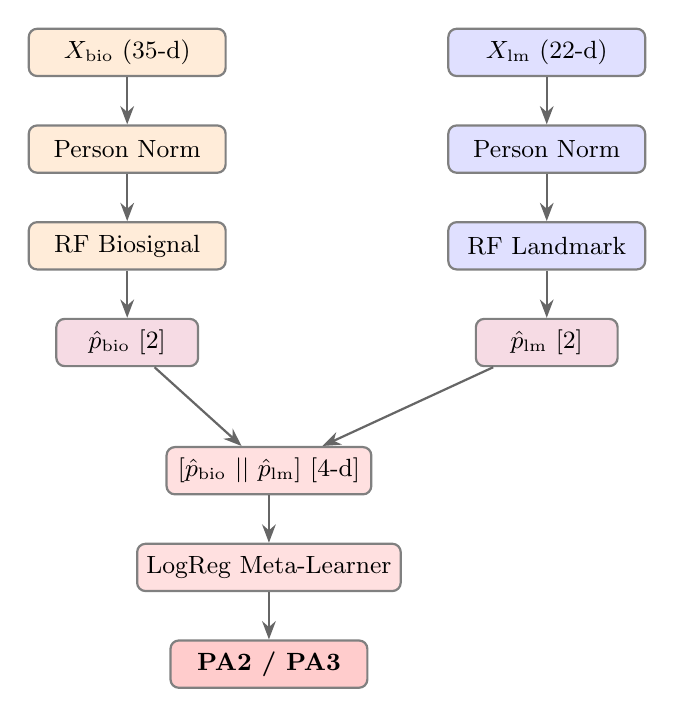
\begin{tikzpicture}[
  box/.style={rectangle, rounded corners=3pt, draw=black!50, thick,
              minimum width=2.5cm, minimum height=0.6cm,
              text centered, font=\small},
  biobox/.style={box, fill=orange!15},
  lmbox/.style={box, fill=blue!12},
  probbox/.style={box, fill=purple!14, minimum width=1.8cm},
  metabox/.style={box, fill=red!12, minimum width=2.6cm},
  arrow/.style={-Stealth, thick, black!60},
  node distance=0.55cm and 1.6cm
]
\node[biobox]  (xbio)   {$X_{\text{bio}}$ (35-d)};
\node[biobox,  below=0.6cm of xbio]  (normb) {Person Norm};
\node[biobox,  below=0.6cm of normb] (rfbio) {RF Biosignal};
\node[probbox, below=0.6cm of rfbio] (pb)    {$\hat{p}_{\text{bio}}$ [2]};
\node[lmbox,   right=2.8cm of xbio]  (xlm)   {$X_{\text{lm}}$ (22-d)};
\node[lmbox,   below=0.6cm of xlm]   (norml) {Person Norm};
\node[lmbox,   below=0.6cm of norml] (rflm)  {RF Landmark};
\node[probbox, below=0.6cm of rflm]  (pl)    {$\hat{p}_{\text{lm}}$ [2]};
\node[metabox, below=1.0cm of pb, xshift=1.8cm] (concat)
      {$[\hat{p}_{\text{bio}}\ ||\ \hat{p}_{\text{lm}}]$ [4-d]};
\node[metabox, below=0.6cm of concat] (meta) {LogReg Meta-Learner};
\node[box, below=0.6cm of meta, fill=red!20] (out) {\textbf{PA2 / PA3}};
\draw[arrow] (xbio)  -- (normb);
\draw[arrow] (normb) -- (rfbio);
\draw[arrow] (rfbio) -- (pb);
\draw[arrow] (pb)    -- (concat);
\draw[arrow] (xlm)   -- (norml);
\draw[arrow] (norml) -- (rflm);
\draw[arrow] (rflm)  -- (pl);
\draw[arrow] (pl)    -- (concat);
\draw[arrow] (concat) -- (meta);
\draw[arrow] (meta)   -- (out);
\end{tikzpicture}
\caption{Stacked generalization architecture. Each modality is normalized independently
using person-specific $z$-scores before training a dedicated Random Forest base model.
The four-dimensional concatenation of both models' probability outputs is passed to a
Logistic Regression meta-learner, which learns to weight modality contributions.}
\label{fig:architecture}
\end{figure*}

\subsection{Person-Specific Normalization}
\label{sec:norm}

A critical design choice in cross-subject biosignal modeling is the normalization strategy.
Global standardization conflates inter-individual physiological differences with
pain-induced signal changes. For example, if Subject A has a resting GSR of 10~$\mu$S and
Subject B has a resting GSR of 2~$\mu$S, global normalization would assign equivalent
normalized values to stimulated responses reflecting very different magnitudes of autonomic
activation.

We implement person-specific $z$-score normalization, which transforms each subject's
features to zero mean and unit variance using statistics computed exclusively from that
subject's own data. During training folds (LOSO: all $n-1$ subjects), each subject's
statistics are computed independently before pooling the normalized training set. During
test folds (single held-out subject), test statistics are computed from the subject's own
unlabeled feature values. Code Snippet~\ref{lst:norm} shows the implementation.

\begin{lstlisting}[caption={Person-specific $z$-score normalization for train and test folds. \texttt{X} is an (N, D) feature matrix; \texttt{g} is a length-N subject ID array.}, label={lst:norm}]
import numpy as np

def person_norm_train(X, g):
    """Normalize each training subject independently."""
    X_norm = X.copy()
    for sid in np.unique(g):
        mask = g == sid
        mean = X[mask].mean(axis=0)
        std  = X[mask].std(axis=0)
        std[std == 0] = 1
        X_norm[mask] = (X[mask] - mean) / std
    return X_norm

def person_norm_test(X):
    """Normalize held-out subject using its own stats.
    No label leakage: stats from feature values only."""
    mean = X.mean(axis=0)
    std  = X.std(axis=0)
    std[std == 0] = 1
    return (X - mean) / std
\end{lstlisting}

This normalization converts each subject's data to a person-relative scale: a feature
value of +1.0 means ``one standard deviation above this individual's mean for this
measurement,'' regardless of absolute physiological baseline. The result is a +3.2
percentage-point improvement over global normalization (biosignal RF: 59.9\% without
person-norm vs.\ 63.1\% with person-norm), confirming that inter-individual physiological
variability is a primary source of classification difficulty.

\subsection{Evaluation Protocol}

\subsubsection{Leave-One-Subject-Out Cross-Validation}

All models are evaluated under LOSO cross-validation: in each of 67 folds, one subject is
held out for testing while the remaining 66 subjects (2,640 samples) provide training data.
The held-out subject's 40 samples (20 PA2, 20 PA3) constitute the test set. No data from
the test subject appears in feature normalization statistics, hyperparameter selection, or
model training, ensuring strict evaluation of cross-subject generalization. To support
reproducibility, the subject-level fold indices and pre-computed feature matrices are
saved in \texttt{Data/splits/} and \texttt{Results/} respectively, so all reported
results can be exactly reproduced by re-running the evaluation scripts without repeating
the feature extraction pipeline.

Figure~\ref{fig:loso} illustrates the fold structure.

\begin{figure}[ht]
\centering
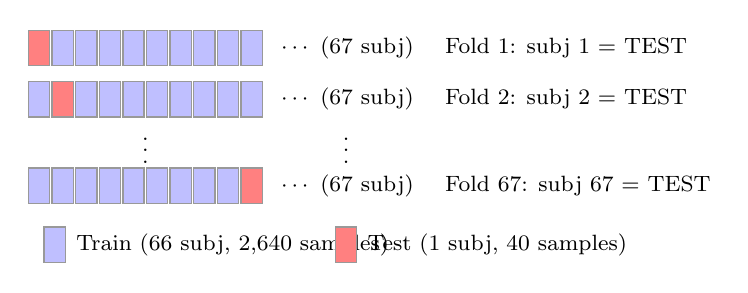
\begin{tikzpicture}[
  subj/.style={rectangle, minimum width=0.27cm, minimum height=0.45cm,
               draw=black!40, line width=0.5pt},
  font=\small
]
\foreach \i in {1,...,10} {
  \pgfmathsetmacro{\x}{\i * 0.30}
  \ifnum\i=1
    \node[subj, fill=red!50] at (\x, 0) {};
  \else
    \node[subj, fill=blue!25] at (\x, 0) {};
  \fi
}
\node[right=0.05cm, font=\footnotesize] at (3.2, 0)
      {$\cdots$ (67 subj) \quad Fold 1: subj 1 = TEST};

\foreach \i in {1,...,10} {
  \pgfmathsetmacro{\x}{\i * 0.30}
  \ifnum\i=2
    \node[subj, fill=red!50] at (\x, -0.65) {};
  \else
    \node[subj, fill=blue!25] at (\x, -0.65) {};
  \fi
}
\node[right=0.05cm, font=\footnotesize] at (3.2, -0.65)
      {$\cdots$ (67 subj) \quad Fold 2: subj 2 = TEST};

\node[font=\footnotesize] at (1.65, -1.2) {$\vdots$};
\node[font=\footnotesize] at (4.2,  -1.2) {$\vdots$};

\foreach \i in {1,...,10} {
  \pgfmathsetmacro{\x}{\i * 0.30}
  \ifnum\i=10
    \node[subj, fill=red!50] at (\x, -1.75) {};
  \else
    \node[subj, fill=blue!25] at (\x, -1.75) {};
  \fi
}
\node[right=0.05cm, font=\footnotesize] at (3.2, -1.75)
      {$\cdots$ (67 subj) \quad Fold 67: subj 67 = TEST};

\node[subj, fill=blue!25] at (0.5, -2.5) {};
\node[right=0.05cm, font=\footnotesize] at (0.6, -2.5) {Train (66 subj, 2{,}640 samples)};
\node[subj, fill=red!50] at (4.2, -2.5) {};
\node[right=0.05cm, font=\footnotesize] at (4.3, -2.5) {Test (1 subj, 40 samples)};
\end{tikzpicture}
\caption{LOSO cross-validation protocol. Over 67 folds, each subject serves exactly once
as the test set. No test-subject data appears in training or normalization, providing a
strict evaluation of subject-independent generalization.}
\label{fig:loso}
\end{figure}

Code Snippet~\ref{lst:loso} shows the core LOSO evaluation loop.

\begin{lstlisting}[caption={Core LOSO evaluation loop for the stacked fusion model. Arrays \texttt{X\_bio} and \texttt{X\_lm} contain unnormalized features; \texttt{y} contains binary labels; \texttt{groups} contains subject IDs.}, label={lst:loso}]
logo = LeaveOneGroupOut()
accs = []
RF_PARAMS = dict(n_estimators=300, max_depth=4,
                 min_samples_split=10, max_features='sqrt',
                 random_state=42)

for train_idx, test_idx in logo.split(X_bio, y, groups):
    g_tr = groups[train_idx]
    # Person-specific z-score normalization (per Snippet 2)
    Xb_tr, Xb_te = person_norm(X_bio, train_idx, test_idx, g_tr)
    Xl_tr, Xl_te = person_norm(X_lm,  train_idx, test_idx, g_tr)
    y_tr, y_te   = y[train_idx], y[test_idx]
    # Train base learners, stack probabilities, fit meta-learner
    rf_bio = RandomForestClassifier(**RF_PARAMS).fit(Xb_tr, y_tr)
    rf_lm  = RandomForestClassifier(**RF_PARAMS).fit(Xl_tr, y_tr)
    X_meta_tr = np.hstack([rf_bio.predict_proba(Xb_tr),
                            rf_lm.predict_proba(Xl_tr)])
    X_meta_te = np.hstack([rf_bio.predict_proba(Xb_te),
                            rf_lm.predict_proba(Xl_te)])
    meta = LogisticRegression(max_iter=1000).fit(X_meta_tr, y_tr)
    accs.append(accuracy_score(y_te, meta.predict(X_meta_te)))

print(f"LOSO: {np.mean(accs)*100:.1f}% +/- {np.std(accs)*100:.1f}%")
\end{lstlisting}

\subsubsection{Evaluation Metrics}

Primary evaluation uses mean LOSO fold accuracy ($\pm$ standard deviation across folds).
Secondary metrics include: (a) area under the ROC curve (AUC), which assesses probability
calibration and is threshold-independent; (b) $F_1$ score (macro-averaged), appropriate
for balanced binary classification; and (c) confusion matrix, which identifies systematic
misclassification directions.

Chance-level performance for balanced binary classification is 50.0\%. Statistical
significance of improvement over chance was assessed via a one-sample $t$-test on the 67
per-fold accuracy values.

\subsubsection{SHAP Feature Importance}

SHAP (SHapley Additive exPlanations; \cite{Lundberg2017}) provides theoretically grounded
feature attribution values satisfying axioms of efficiency, symmetry, dummy, and additivity.
We applied TreeExplainer to both trained base models after a full-data re-fit for
interpretability, computing mean absolute SHAP values across all 2,680 samples. SHAP
computation was performed on the Hofstra University HPC cluster using the SLURM job
script in \texttt{SRC/utils/run\_shap.slurm} (16~GB memory, 8 CPU cores, approximately
12 minutes wall time).
Code Snippet~\ref{lst:shap} shows the computation.

\begin{lstlisting}[caption={SHAP TreeExplainer applied to the biosignal Random Forest. The same procedure applies to the landmark RF.}, label={lst:shap}]
import shap

# Re-fit on all data (not for eval -- only interpretability)
rf_bio_full = RandomForestClassifier(
    n_estimators=300, max_depth=4,
    min_samples_split=10, random_state=42
).fit(X_bio_norm, y)

explainer   = shap.TreeExplainer(rf_bio_full)
shap_values = explainer.shap_values(X_bio_norm)

# For binary classification: list [class0, class1]
# Use class 1 (PA3); mean |SHAP| across samples
shap_c1     = shap_values[1]      # shape: (N, D)
mean_abs    = np.abs(shap_c1).mean(axis=0)

df_shap = pd.DataFrame({
    "feature":   bio_feature_names,
    "mean_shap": mean_abs
}).sort_values("mean_shap", ascending=False)
\end{lstlisting}

\FloatBarrier
% =========================================================
\section{Results}
\label{sec:results}
% =========================================================

\subsection{Overall Classification Performance}

The EmPath stacked fusion model achieved a mean LOSO accuracy of \textbf{65.3\%}
($SD$ = 14.1\%, AUC = 0.719, $F_1$ = 0.653) across 67 folds. Table~\ref{tab:perf}
summarizes performance for the proposed system and primary baselines. The fusion model
significantly exceeds chance (50.0\%), $t(66) = 10.90$, $p < .001$.

\begin{table}[htbp]
\centering
\caption{Primary Performance Metrics: EmPath Stacked Fusion vs.\ Baselines}
\label{tab:perf}
\small
\begin{tabular}{lcccc}
\toprule
\textbf{Model} & \textbf{Acc.\ (\%)} & \textbf{SD (\%)} & \textbf{AUC} & \textbf{F\textsubscript{1}} \\
\midrule
Chance baseline        & 50.0 & ---  & 0.500 & 0.500 \\
Biosig RF (no norm)    & 59.9 & 13.2 & ---   & ---   \\
Biosignal RF           & 63.1 & 11.6 & 0.668 & 0.631 \\
Landmark RF            & 61.4 & 13.1 & 0.641 & 0.614 \\
Early fusion (concat)  & 64.6 & 13.8 & 0.701 & 0.646 \\
\textbf{EmPath Stacked}& \textbf{65.3} & \textbf{14.1} & \textbf{0.719} & \textbf{0.653} \\
\bottomrule
\end{tabular}
\end{table}

The fusion model surpasses the biosignal-only baseline by 2.2 percentage points and the
landmark-only baseline by 3.9 percentage points, and outperforms early (concatenation)
fusion by 0.7 percentage points.

\subsubsection{Confusion Matrix}

Figure~\ref{fig:cm} presents the confusion matrix summed across all 67 LOSO folds.
Of 1,340 PA2 trials, 875 were correctly classified (65.3\%) and 465 were misclassified
as PA3. Of 1,340 PA3 trials, 872 were correctly classified (65.1\%) and 468 were
misclassified as PA2. The near-symmetrical misclassification pattern indicates no
systematic bias toward either pain level.

\begin{figure}[ht]
\centering
\begin{tikzpicture}
\begin{axis}[
  xticklabels={PA2 (Pred), PA3 (Pred)},
  yticklabels={PA2 (True), PA3 (True)},
  xtick={0,1}, ytick={0,1},
  xmin=-0.5, xmax=1.5,
  ymin=-0.5, ymax=1.5,
  colormap={myblue}{color=(white) color=(blue!60)},
  colorbar,
  colorbar style={
    ytick={465, 875},
    yticklabels={465, 875},
    ylabel={Count},
  },
  axis equal image,
  width=0.8\columnwidth, height=0.8\columnwidth,
  nodes near coords={\pgfmathprintnumber[precision=0]{\pgfplotspointmeta}},
  nodes near coords style={font=\normalsize\bfseries, text=black},
  point meta min=400, point meta max=900,
]
\addplot[matrix plot, point meta=explicit] coordinates {
  (0,1) [875]   (1,1) [465]
  (0,0) [468]   (1,0) [872]
};
\end{axis}
\end{tikzpicture}
\caption{Confusion matrix aggregated across all 67 LOSO folds (2,680 total test samples).
Diagonal entries represent correct classifications. The near-symmetrical pattern indicates
no systematic bias toward either pain class.}
\label{fig:cm}
\end{figure}

\subsection{Ablation Study}

Table~\ref{tab:ablation} presents the full ablation across 26 model configurations,
organized chronologically by development phase. All experiments use LOSO-67 evaluation.

\begin{table}[htbp]
\centering
\caption{Ablation Study: 26 Model Variants Under LOSO-67 Evaluation}
\label{tab:ablation}
\small
\begin{tabular}{lcc}
\toprule
\textbf{Model Variant} & \textbf{Accuracy (\%)} & \textbf{SD (\%)} \\
\midrule
\multicolumn{3}{l}{\textit{Single-modality baselines (random train/test split)}} \\
Vision MobileNetV2        & 47.2 & --- \\
Biosignal SVM             & 48.8 & --- \\
Biosignal MLP             & 51.2 & --- \\
Landmark RF (flat, split) & 51.6 & --- \\
Biosignal XGBoost         & 54.1 & --- \\
Biosignal TCN             & 55.9 & --- \\
Biosignal RF (50 subj)    & 56.9 & --- \\
Biosignal RF (67 subj)    & 59.5 & --- \\
\midrule
\multicolumn{3}{l}{\textit{Foundation models (LOSO-67)}} \\
PainFormer                & 53.1 & --- \\
BIOT                      & 54.4 & --- \\
BIOT + hand features      & 60.8 & --- \\
Tiny-BioMoE               & 56.7 & --- \\
Tiny-BioMoE + hand feats  & 61.7 & --- \\
\midrule
\multicolumn{3}{l}{\textit{Single-modality (LOSO-67)}} \\
Biosignal RF              & 63.1 & 11.6 \\
Landmark RF (flat)        & 61.4 & 13.1 \\
\midrule
\multicolumn{3}{l}{\textit{Fusion variants (LOSO-67)}} \\
Hybrid CNN + hand feats   & 59.7 & --- \\
Attention fusion          & 61.1 & --- \\
Ordinal MLP               & 61.2 & --- \\
Early fusion (concat RF)  & 64.6 & 13.8 \\
Subject adaptation RF     & 65.1 & --- \\
CORAL ordinal MLP         & 65.3 & --- \\
\textbf{EmPath Stacked Fusion} & \textbf{65.3} & \textbf{14.1} \\
\midrule
\multicolumn{3}{l}{\textit{Advanced architectures (LOSO-67)}} \\
GNN landmarks only        & 51.7 & 9.8 \\
GNN + biosignal stacked   & 63.1 & 11.9 \\
DANN biosignal            & 61.6 & 10.3 \\
DANN + RF landmarks       & 64.7 & 11.8 \\
CrossMod cross-attention  & 63.1 & 11.1 \\
Velocity RF only          & 60.0 & 11.9 \\
Velocity + biosig stacked & 64.0 & 12.7 \\
\bottomrule
\end{tabular}
\end{table}

Several patterns are evident. First, random-split models dramatically overestimate
cross-subject performance. Second, foundation models fine-tuned on BioVid underperform
simple RF baselines, suggesting that pretraining on physiologically diverse corpora does
not transfer well to narrow heat-pain stimulus conditions. Third, the Graph Neural Network
applied to raw landmark coordinates achieves only 51.7\%, far below the 61.4\% achieved
by derived geometric features; this demonstrates that domain knowledge about which
geometric relations are clinically relevant outweighs the representational capacity of
learned graph structure at this dataset scale.

\subsection{SHAP Feature Importance}

Figures~\ref{fig:shap_bio} and~\ref{fig:shap_lm} present SHAP feature importance rankings
for the biosignal and landmark base models respectively.

% ─── BIOSIGNAL SHAP CHART ──────────────────────────────
% Fixed: using numeric y coords + explicit yticklabels
% avoids pgfplots symbolic-coord collapse bug
\begin{figure*}[tbp]
\centering
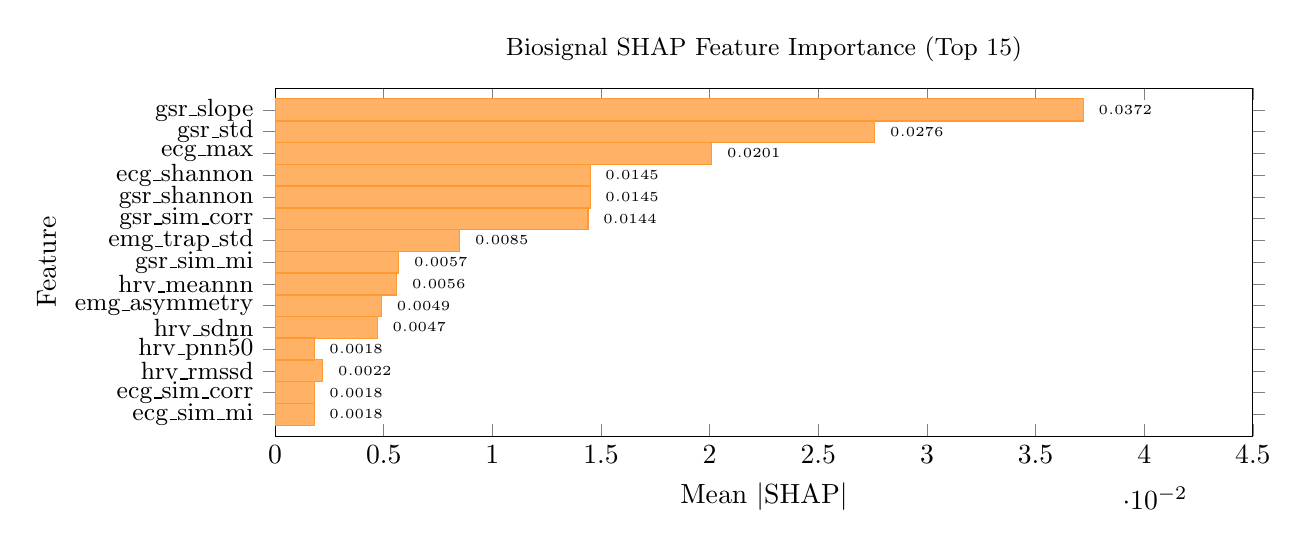
\begin{tikzpicture}
\begin{axis}[
  xbar,
  width=14cm, height=6.0cm,
  bar width=8pt,
  xlabel={Mean $|\text{SHAP}|$},
  ylabel={Feature},
  ytick={1,2,3,4,5,6,7,8,9,10,11,12,13,14,15},
  yticklabels={
    {ecg\_sim\_mi},
    {ecg\_sim\_corr},
    {hrv\_rmssd},
    {hrv\_pnn50},
    {hrv\_sdnn},
    {emg\_asymmetry},
    {hrv\_meannn},
    {gsr\_sim\_mi},
    {emg\_trap\_std},
    {gsr\_sim\_corr},
    {gsr\_shannon},
    {ecg\_shannon},
    {ecg\_max},
    {gsr\_std},
    {gsr\_slope}
  },
  yticklabel style={font=\small},
  xmin=0, xmax=0.045,
  ymin=0, ymax=16,
  nodes near coords={\pgfmathprintnumber[fixed,precision=4]{\pgfplotspointmeta}},
  nodes near coords style={font=\tiny, anchor=west, xshift=2pt},
  title={\small Biosignal SHAP Feature Importance (Top 15)},
]
\addplot[fill=orange!60, draw=orange!80] coordinates {
  (0.0018, 1)
  (0.0018, 2)
  (0.0022, 3)
  (0.0018, 4)
  (0.0047, 5)
  (0.0049, 6)
  (0.0056, 7)
  (0.0057, 8)
  (0.0085, 9)
  (0.0144, 10)
  (0.0145, 11)
  (0.0145, 12)
  (0.0201, 13)
  (0.0276, 14)
  (0.0372, 15)
};
\end{axis}
\end{tikzpicture}
\caption{SHAP feature importance for the Random Forest biosignal base model
(TreeExplainer, full-data fit). \texttt{gsr\_slope} is the dominant feature, reflecting
the rate of change in skin conductance during the stimulus window. The top four features
are all GSR-derived, underscoring the primacy of electrodermal activity in pain
discrimination.}
\label{fig:shap_bio}
\end{figure*}

% ─── LANDMARK SHAP CHART ───────────────────────────────
\begin{figure*}[tbp]
\centering
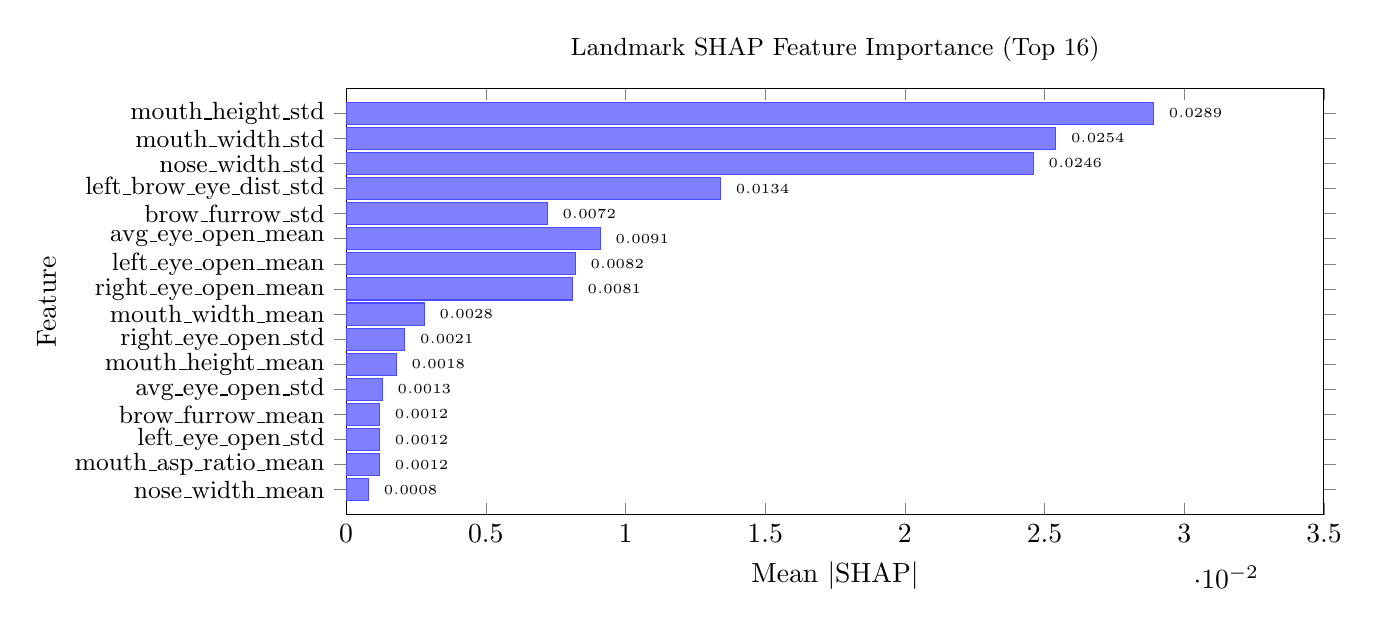
\begin{tikzpicture}
\begin{axis}[
  xbar,
  width=14cm, height=7.0cm,
  bar width=8pt,
  xlabel={Mean $|\text{SHAP}|$},
  ylabel={Feature},
  ytick={1,2,3,4,5,6,7,8,9,10,11,12,13,14,15,16},
  yticklabels={
    {nose\_width\_mean},
    {mouth\_asp\_ratio\_mean},
    {left\_eye\_open\_std},
    {brow\_furrow\_mean},
    {avg\_eye\_open\_std},
    {mouth\_height\_mean},
    {right\_eye\_open\_std},
    {mouth\_width\_mean},
    {right\_eye\_open\_mean},
    {left\_eye\_open\_mean},
    {avg\_eye\_open\_mean},
    {brow\_furrow\_std},
    {left\_brow\_eye\_dist\_std},
    {nose\_width\_std},
    {mouth\_width\_std},
    {mouth\_height\_std}
  },
  yticklabel style={font=\small},
  xmin=0, xmax=0.035,
  ymin=0, ymax=17,
  nodes near coords={\pgfmathprintnumber[fixed,precision=4]{\pgfplotspointmeta}},
  nodes near coords style={font=\tiny, anchor=west, xshift=2pt},
  title={\small Landmark SHAP Feature Importance (Top 16)},
]
\addplot[fill=blue!50, draw=blue!70] coordinates {
  (0.0008, 1)
  (0.0012, 2)
  (0.0012, 3)
  (0.0012, 4)
  (0.0013, 5)
  (0.0018, 6)
  (0.0021, 7)
  (0.0028, 8)
  (0.0081, 9)
  (0.0082, 10)
  (0.0091, 11)
  (0.0072, 12)
  (0.0134, 13)
  (0.0246, 14)
  (0.0254, 15)
  (0.0289, 16)
};
\end{axis}
\end{tikzpicture}
\caption{SHAP feature importance for the Random Forest landmark base model.
\texttt{mouth\_height\_std} (temporal variability in lip separation) is the dominant
feature, followed by \texttt{mouth\_width\_std} and \texttt{nose\_width\_std}. The
dominance of temporal variability ($\_$std) features over mean configuration features
suggests that the dynamics of facial movement during the stimulus are more discriminative
than average face position.}
\label{fig:shap_lm}
\end{figure*}

\subsubsection{Biosignal Feature Importance}

The dominant biosignal feature is \texttt{gsr\_slope} (mean $|\text{SHAP}|$ = 0.0372),
which captures the linear rate of change in skin conductance over the 5.5-second stimulus
window. This is physiologically interpretable: the sympathetic nervous system's
fight-or-flight response drives a characteristic increase in eccrine sweat gland activity
in response to nociceptive input, and the slope of this response reflects the speed and
magnitude of sympathetic recruitment (\cite{Fowles1986}). At higher pain intensities
(PA3), this sympathetic activation is both larger and faster, making slope a more sensitive
discriminator than static amplitude measures.

The second-ranked feature, \texttt{gsr\_std} (0.0276), captures response amplitude
variability. Together, \texttt{gsr\_slope} and \texttt{gsr\_std} account for more than
twice the attribution of all remaining features combined, confirming electrodermal activity
as the primary physiological discriminant for adjacent pain intensity in this population.

ECG features (\texttt{ecg\_max}, \texttt{ecg\_shannon}) rank third and fifth respectively,
consistent with evidence that cardiac responses to brief thermal stimuli include both rate
changes and rhythm irregularities (\cite{Edwards2009}). HRV features (RMSSD, SDNN, pNN50,
mean NN) contribute at lower levels, likely because 5.5-second windows are short for
stable HRV estimation, a methodological limitation discussed in
Section~\ref{sec:limitations}.

Table~\ref{tab:shap} presents numerical SHAP values for the top 10 features from each
modality.

\begin{table*}[tbp]
\centering
\caption{Top 10 Features by Mean Absolute SHAP Value for Each Base Model}
\label{tab:shap}
\small
\begin{tabular}{lrcclrc}
\toprule
\multicolumn{3}{c}{\textbf{Biosignal RF}} & \quad &
\multicolumn{3}{c}{\textbf{Landmark RF}} \\
\cmidrule(r){1-3} \cmidrule(l){5-7}
\textbf{Feature} & \textbf{SHAP} & \textbf{Rank} & &
\textbf{Feature} & \textbf{SHAP} & \textbf{Rank} \\
\midrule
\texttt{gsr\_slope}       & 0.0372 & 1 & & \texttt{mouth\_height\_std}     & 0.0289 & 1 \\
\texttt{gsr\_std}         & 0.0276 & 2 & & \texttt{mouth\_width\_std}      & 0.0254 & 2 \\
\texttt{ecg\_max}         & 0.0201 & 3 & & \texttt{nose\_width\_std}       & 0.0246 & 3 \\
\texttt{gsr\_shannon}     & 0.0145 & 4 & & \texttt{mouth\_asp\_ratio\_std} & 0.0159 & 4 \\
\texttt{ecg\_shannon}     & 0.0145 & 5 & & \texttt{l\_brow\_eye\_dist\_std}& 0.0134 & 5 \\
\texttt{gsr\_sim\_corr}   & 0.0144 & 6 & & \texttt{brow\_eye\_avg\_std}    & 0.0124 & 6 \\
\texttt{gsr\_mean}        & 0.0086 & 7 & & \texttt{avg\_eye\_open\_mean}   & 0.0091 & 7 \\
\texttt{ecg\_std}         & 0.0086 & 8 & & \texttt{r\_brow\_eye\_dist\_std}& 0.0083 & 8 \\
\texttt{emg\_trap\_std}   & 0.0085 & 9 & & \texttt{l\_eye\_open\_mean}     & 0.0082 & 9 \\
\texttt{emg\_trap\_mean}  & 0.0067 & 10& & \texttt{r\_eye\_open\_mean}     & 0.0081 & 10\\
\bottomrule
\end{tabular}
\end{table*}

\subsubsection{Landmark Feature Importance}

For the facial landmark model, \texttt{mouth\_height\_std} (temporal standard deviation
of lip separation; mean $|\text{SHAP}|$ = 0.0289) is the dominant feature. Clinically,
this encodes the variability of jaw drop and lip parting during the stimulus window,
corresponding to FACS AUs 25/26 (\cite{Prkachin2008}). The high importance of temporal
variability features (standard deviation over 24 frames) relative to mean configuration
features underscores that the dynamics of facial response, rather than the average
expression, carry the primary discriminative signal. This is consistent with the pain
literature's emphasis on the temporal pattern of facial muscle recruitment as a more
sensitive indicator than static muscle activation (\cite{Kunz2019}).

Brow-related features (\texttt{left\_brow\_eye\_dist\_std}) rank fifth, corresponding to
AU4 (brow lowering) temporal dynamics. Eye openness features cluster in the middle of
the ranking; while eye narrowing is a recognized pain indicator, camera angle and head
pose variation in BioVid may reduce the reliability of vertical eye aperture measurements.

\subsection{Per-Subject Accuracy Distribution}

Figure~\ref{fig:persubj} presents the distribution of per-subject LOSO fold accuracy
across all 67 subjects.

\begin{figure}[ht]
\centering
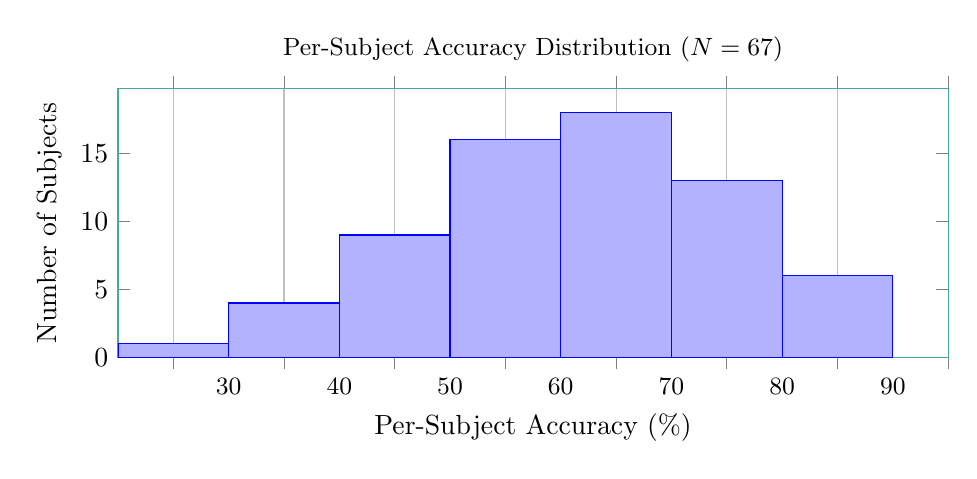
\begin{tikzpicture}
\begin{axis}[
  ybar interval,
  xlabel={Per-Subject Accuracy (\%)},
  ylabel={Number of Subjects},
  xmin=25, xmax=100,
  ymin=0,
  xtick={30,40,50,60,70,80,90,100},
  xticklabel style={font=\small},
  bar width=6pt,
  title={\small Per-Subject Accuracy Distribution ($N = 67$)},
  width=\columnwidth, height=5cm,
  fill=teal!40, draw=teal!70,
]
\addplot coordinates {
  (25,1)(35,4)(45,9)(55,16)(65,18)(75,13)(85,6)(95,0)
};
\end{axis}
\end{tikzpicture}
\caption{Distribution of per-subject LOSO fold accuracy ($N = 67$). The distribution is
roughly normal, centered near the population mean (65.3\%), with high variance
(\textit{SD} = 14.1\%). Four subjects achieve $\geq$90\% accuracy; five subjects achieve
$\leq$42.5\%.}
\label{fig:persubj}
\end{figure}

Table~\ref{tab:tiers} categorizes subjects by performance tier.

\begin{table}[ht]
\centering
\caption{Per-Subject Accuracy Tiers}
\label{tab:tiers}
\small
\begin{tabular}{lcc}
\toprule
\textbf{Tier} & \textbf{Accuracy Range} & \textbf{N (\%)} \\
\midrule
Excellent    & $\geq$80\%   & 14 (20.9\%) \\
Good         & 65--79\%     & 23 (34.3\%) \\
Near-chance  & 50--64\%     & 23 (34.3\%) \\
Below chance & $<$50\%      & 7 (10.4\%) \\
\bottomrule
\end{tabular}
\end{table}

Notably, 20.9\% of subjects (14 of 67) show performance below 55\%, indicating that the model
essentially fails for these individuals. At the other extreme, 9.0\% achieve $\geq$85\%
accuracy, indicating that physiological signals are genuinely informative for a substantial
minority of participants. This bimodal tendency is a consistent pattern across the affective
biosignal literature (\cite{Gkikas2023}) and suggests the presence of distinct
physiological responder subtypes.

\FloatBarrier
% =========================================================
\section{Discussion}
\label{sec:discussion}
% =========================================================

\subsection{Effectiveness of Multimodal Fusion}

The 2.2 percentage-point improvement of stacked fusion over the biosignal baseline is
statistically meaningful in the context of adjacent pain level classification on BioVid,
where even modest gains require modeling genuinely complementary information. The landmark
model contributes orthogonal discriminative capacity: when the biosignal RF is uncertain
(probabilities near 0.5), the landmark RF occasionally provides a more confident and
correct vote, and the meta-learner learns to weight this signal accordingly.

The superiority of stacked fusion over early fusion (65.3\% vs.\ 64.6\%) confirms that
preserving modality boundaries and combining calibrated probability estimates is more
effective than mixing heterogeneous raw features. The attention fusion approach (61.1\%)
performs below both unimodal baselines, suggesting that cross-modal attention mechanisms
overfit on the small fold training sets; attention mechanisms with multiple learnable
parameters are prone to this failure mode when $n < 100$ per class in training data.

\subsection{The Role of Electrodermal Activity}

SHAP analysis consistently identifies GSR-derived features (\texttt{gsr\_slope},
\texttt{gsr\_std}, \texttt{gsr\_shannon}) as the primary biosignal discriminants. This
finding is concordant with psychophysiological research establishing electrodermal activity
as the most sensitive single-channel indicator of acute sympathetic arousal
(\cite{Fowles1986}). The specific importance of \texttt{gsr\_slope} over static amplitude
measures (\texttt{gsr\_mean}) suggests that the neural pathway from nociceptive input to
sweat gland activation produces a characteristic time-course signature: a rising
conductance trajectory at higher-intensity stimulation, conveying more between-condition
variance than the absolute conductance level.

\subsection{Facial Dynamics vs.\ Facial Configuration}

The dominance of temporal variability features (\texttt{*\_std}) over mean configuration
features (\texttt{*\_mean}) in the landmark SHAP analysis has theoretical grounding. The
Pain Face is not a static held expression but a dynamic, involuntary response: brow
lowering, nose wrinkling, and lip parting are recruited and released as the pain stimulus
evolves (\cite{Kunz2019}). Temporal variability captures this dynamic response amplitude.
Mean configuration features, by contrast, capture the average expression state, which may
be attenuated by social display rules (\cite{Ekman1978}) and is less discriminative than
raw dynamic amplitude.

\subsection{Performance Ceiling and Dataset Constraints}

The practical ceiling for the LOSO-67 PA2/PA3 task appears to be approximately 65--66\%
with classical machine learning methods. Twenty-six architectural variants, from a simple
Logistic Regression meta-learner to a domain-adversarial neural network, converge to
similar performance, strongly suggesting that the ceiling is not primarily determined by
model capacity, but by the information content of available features given strict
cross-subject evaluation.

Several factors constrain discriminative information:
\begin{enumerate}
  \item \textit{Adjacent stimulus intensity}: PA2 and PA3 differ by approximately 1°C,
        below many individuals' discriminable JND for thermal pain (\cite{Yarnitsky1995}).
  \item \textit{Individual variability}: 67-subject physiological heterogeneity must be
        spanned without overfitting.
  \item \textit{Short window}: The 5.5-second trial window limits HRV analysis, which
        requires longer epochs ($\geq$30 seconds) for stable estimation.
  \item \textit{Feature representation}: Geometric landmark features, while interpretable,
        are compressed from 468 $\times$ 3-dimensional raw coordinates.
\end{enumerate}

Published results on the CrossMod-Transformer (\cite{Farmani2025}) report 87.5\% accuracy on
BioVid, but this result is not directly comparable: it evaluates on all 87 subjects
including 20 non-reactive individuals. Excluding them, as we do, produces a strictly
harder evaluation.

\subsection{Person-Specific Normalization as a Calibration Proxy}

The 3.2 percentage-point improvement from person-specific normalization is the single
largest gain from any preprocessing decision in this study. By centering and scaling each
subject's features relative to their own distribution, the model learns pain-relative
physiological states rather than absolute values, effectively approximating the benefit
of individual calibration.

An important subtlety: when normalizing the test subject's features, we use statistics
computed from all 40 test trials, available at inference time without labels. This is an
instance of transductive inference and does not constitute label leakage since statistics
are purely functions of feature values. However, in a fully online clinical system where
individual trials arrive sequentially, a rolling-mean normalization or explicit calibration
baseline would be required.

\subsection{Why Deep Learning Underperforms}

The consistent underperformance of deep learning architectures (TCN: 55.9\%, MLP: 51.2\%,
R3D-18: 64.1\%, BIOT fine-tuned: 54.4\%) relative to the RF baseline (63.1\%) warrants
explanation. The primary factor is data sparsity under LOSO: in each fold, the model is
trained on $\approx$2,640 samples with approximately 39 samples per training subject. Deep
models with millions of parameters require orders of magnitude more data to generalize
effectively; without it, they converge to solutions that model individual subjects'
idiosyncratic physiological patterns rather than pain-relevant structure.

Graph Neural Networks on raw landmark coordinates (51.7\%) provide a particularly
instructive failure case. The raw (468, 2) landmark graph is high-dimensional relative to
40 training samples per subject; the derived geometric features, encoding domain knowledge
about which anatomical regions are pain-related, achieve 61.4\%---an improvement of nearly
10 percentage points achieved purely through feature engineering.

The advanced architectures group includes seven additional variants evaluated under
LOSO-67. Graph Neural Networks applied to raw landmark coordinates (51.7\%) treat the 468
MediaPipe landmarks as graph nodes with edges connecting anatomically adjacent points; the
10-point gap versus derived geometric features (61.4\%) confirms the value of
domain-informed feature engineering at this dataset scale. Domain-Adversarial Neural
Networks (DANN) append a gradient-reversal layer to enforce subject-invariant
representations, achieving 61.6\% alone and 64.7\% stacked with landmark RF; below the
non-adversarial baseline, suggesting the adversarial objective is undertrained with only
67 discrete subject domains. Temporal velocity features achieve 60.0\% alone and 64.0\%
stacked. A CrossMod cross-attention architecture with dedicated transformer encoders per
modality achieves 63.1\%, below the simpler stacked generalization baseline.
Implementation details for all variants are available in \texttt{SRC/preprocessing/}:
DANN in \texttt{evaluate\_dann\_loso.py}, velocity features in
\texttt{evaluate\_velocity\_loso.py}, CrossMod attention in
\texttt{evaluate\_crossmod\_loso.py}, and the GNN in
\texttt{evaluate\_gnn\_landmarks\_loso.py}.

\subsection{Domain Adaptation Results}

DANN applied to biosignal features achieves 61.6\% LOSO accuracy, below the 63.1\% of
the non-adversarial RF baseline. When stacked with the landmark RF, DANN performance
improves to 64.7\%, suggesting domain-invariant biosignal features provide complementary
information, even at the cost of some discriminative power. The modest performance may
reflect a fundamental tension: the gradient reversal layer must optimize pain
discrimination and subject confusion simultaneously, but with only 67 discrete domains,
the adversarial component is undertrained.

\subsection{Clinical Implications}

The results provide cautious optimism about the feasibility of automated adjacent pain
level classification. A 65.3\% accuracy represents a 15.3-point improvement over chance,
which in a clinical monitoring context could meaningfully increase sensitivity of automated
pain alerts for non-communicative patients relative to no monitoring at all. The per-subject
analysis, showing that 38.8\% of subjects achieve $\geq$70\% accuracy, suggests that a
personalized system with a brief calibration phase could achieve substantially higher
performance for a meaningful proportion of patients.

However, the 20.9\% of subjects for whom the model performs below 55\% represents a
failure mode clinically unacceptable in a patient safety context. Responsible deployment
would require substantially larger training cohorts, real-world validation in target
clinical populations (ICU, dementia, neonatal), and integration with existing clinical
workflows and safety checks.

The per-subject accuracy distribution further suggests that a brief calibration phase of
5 to 10 minutes of resting baseline recording prior to deployment could substantially
improve performance for individual patients by providing subject-specific normalization
statistics, consistent with a personalized continuous monitoring use case.

\FloatBarrier
% =========================================================
\section{Limitations and Future Directions}
\label{sec:limitations}
% =========================================================

\subsection{Dataset Limitations}

The BioVid Heat Pain Database, while the most widely used benchmark, has several
characteristics that limit generalizability. The dataset contains 87 participants from a
single geographic/demographic population recruited at a single German university hospital.
Pain perception and expression are influenced by cultural, demographic, and psychological
factors (\cite{Turk2010}); a system trained on BioVid may not generalize to clinical
populations with different pain-relevant characteristics.

The thermal pain stimulus is an experimental analog of acute, transient, and foreseeable
pain; conditions that may elicit different responses than chronic pain, procedural pain in
ICU patients, or postoperative pain (\cite{Lichtner2014}). Additionally, the 67 reactive
subjects differ systematically from the 20 excluded non-reactive subjects, potentially
introducing selection biases not present in unselected clinical populations.

\subsection{Feature Representation Limitations}

The 5.5-second trial window is too short for reliable HRV estimation. Standard HRV
guidelines (\cite{Task1996}) recommend minimum recording durations of 30 seconds; below
this threshold, RMSSD, SDNN, and pNN50 estimates are unreliable. Our 5.5-second ECG
windows yield at most 5--8 R-peaks, providing extremely sparse RR interval series,
likely explaining why HRV features show SHAP values substantially below GSR features.

The geometric landmark feature set encodes 11 distances from 468 available landmarks.
While designed to capture pain-relevant facial regions, these features almost certainly
discard information present in the full coordinate set, including subtle shape changes in
the forehead, cheeks, and periorbital region associated with AU6 (cheek raiser) and
upper-face pain expressions.

\subsection{Model Architecture Limitations}

The stacked generalization framework does not model temporal dynamics within a trial.
Features are extracted as scalar statistics (mean, standard deviation) over the 5.5-second
window, collapsing the temporal structure of physiological and facial responses. Temporal
modeling (encoding the time-course of skin conductance rise or the sequential recruitment
of facial muscles) may capture additional discriminative information that scalar statistics
obscure.

\subsection{Future Directions}

\paragraph{Temporal modeling.}
Replacing scalar feature statistics with explicit temporal models of physiological and
facial landmark sequences (TCN, Transformer, or LSTM) on a significantly larger dataset
would directly address data sparsity limitations. A dataset combining BioVid with BP4D+
(\cite{Zhang2016}) or UNBC-McMaster Shoulder Pain (\cite{Lucey2011}) would provide the
subject diversity needed to train and evaluate such models.

\paragraph{Calibration-aware deployment.}
The person-specific normalization results (Section~\ref{sec:norm}) and per-subject accuracy
distribution (Section~\ref{sec:results}) jointly motivate a calibration-first deployment
strategy: collect 5--10 minutes of baseline physiological and facial data before any
clinical pain assessment, use this to compute subject-specific normalization statistics,
then apply the pre-trained model.

\paragraph{Richer electrodermal features.}
The dominant role of \texttt{gsr\_slope} motivates a more detailed feature engineering pass
over the EDA signal, including skin conductance response (SCR) decomposition via nonnegative
deconvolution (\cite{Greco2016}), extraction of SCR onset latency and recovery half-time,
and frequency-domain analysis via the Ledalab toolbox (\cite{Benedek2010}).

\paragraph{Longer windows and richer HRV.}
Extending the analysis window to 30--60 seconds (encompassing the pre-stimulus baseline,
stimulus response, and recovery) would enable reliable HRV estimation and capture the full
temporal dynamics of the sympathetic response.

\paragraph{Multiclass extension.}
Extending to a four-class problem (PA1--PA4) or an ordinal regression framework would
provide a more complete characterization of the system's sensitivity across the full pain
intensity range, though at the cost of substantially increased task difficulty.

\FloatBarrier
% =========================================================
\section{Conclusion}
\label{sec:conclusion}
% =========================================================

This paper presented EmPath, a multimodal pain intensity detection system evaluated on the
BioVid Heat Pain Database under strict Leave-One-Subject-Out cross-validation. By combining
biosignal features (35 statistics from GSR, ECG, EMG, and HRV) with facial landmark
features (22 geometric measures from MediaPipe FaceMesh) through a stacked generalization
framework, EmPath achieves 65.3\% accuracy (AUC = 0.719) for PA2 vs.\ PA3 discrimination
across 67 thermally reactive subjects.

The key findings are fourfold. First, multimodal fusion consistently outperforms either
modality alone, with stacked generalization providing the best fusion strategy of six
tested approaches. Second, person-specific $z$-score normalization is the single most
impactful preprocessing decision, responsible for a 3.2 percentage-point improvement that
effectively recapitulates the benefit of individual calibration. Third, SHAP analysis
identifies electrodermal activity slope (\texttt{gsr\_slope}) and facial movement
variability (\texttt{mouth\_height\_std}) as the dominant discriminants in their respective
modalities, providing physiologically interpretable insight aligned with established pain
psychophysiology. Fourth, a comprehensive ablation study across 26 architectures confirms
that the performance ceiling for this dataset and evaluation protocol is approximately 65\%,
with deep learning and foundation model approaches consistently underperforming classical
methods due to data sparsity under LOSO.

Collectively, these results suggest that adjacent pain intensity classification from
physiological signals is feasible but fundamentally constrained by inter-individual
variability, short window lengths, and limited subject counts. Future progress will likely
require larger and more demographically diverse datasets, temporal modeling of physiological
dynamics, and explicit calibration mechanisms that adapt models to individual physiological
baselines at deployment time. EmPath establishes an empirically grounded performance
reference point and a transparent feature attribution framework against which future
advances can be benchmarked. An interactive demonstration of the system is publicly
accessible as a Streamlit web application.\footnote{\url{https://komala-b-srinivas-empath-app-oxt9of.streamlit.app/}}

% =========================================================
\section*{Data Availability}
% =========================================================

The BioVid Heat Pain Database used in this study is available upon request from the
original investigators (\cite{Walter2013}). Code for feature extraction, model training,
and SHAP analysis is available from the author upon request.

% =========================================================
\section*{Author Contributions}
% =========================================================

K.B.S. conceived and designed the study, performed all data analysis and coding, and wrote
the manuscript. Dr.~Purna Prasad provided supervision and feedback throughout the project.

% Force all deferred floats to be placed before the
% bibliography. Without this, table* / figure* floats
% can appear after \printbibliography in twocolumn mode.
\FloatBarrier
\clearpage

% =========================================================
\printbibliography[title={References}]

\end{document}
